\section{Results}\label{sec:res}
\subsection{Two-body system}
\begin{figure}[H]
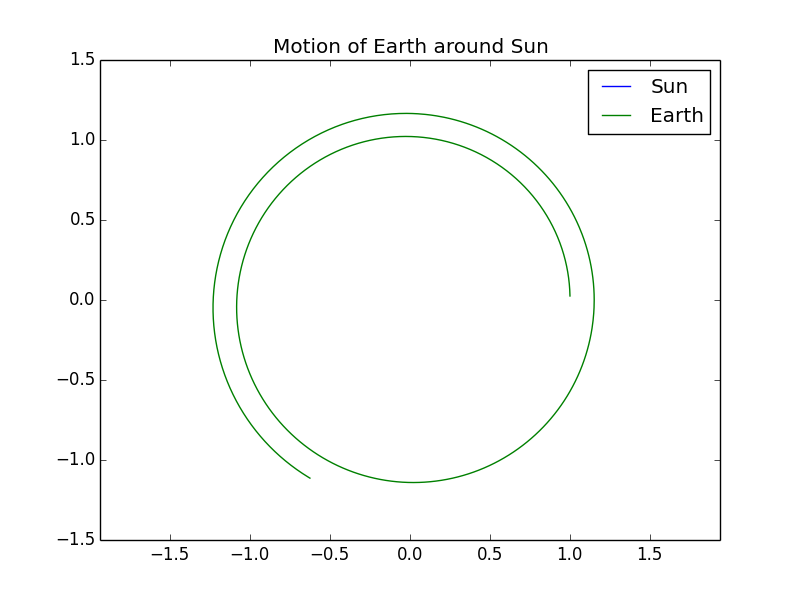
\includegraphics[scale=0.7]{figures/earth_sun_euler}
\caption{The plot shows the simulated orbit of the Earth around the Sun using the forward Euler integration method. The motion is simulated for two years, with $\Delta t = 0.002$ years.}
\end{figure}


\begin{figure}[H]
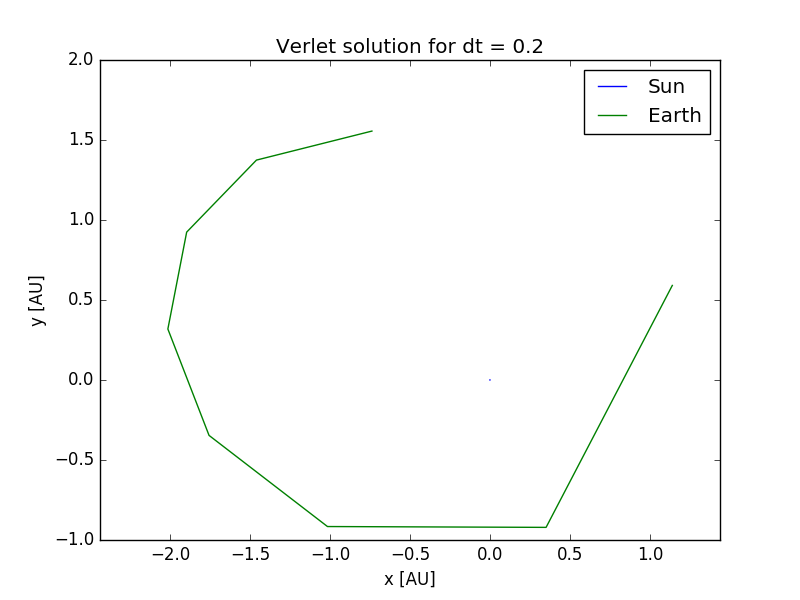
\includegraphics[scale=0.7]{figures/verlet_02}
\caption{The plot shows the simulated orbit of the Earth around the Sun using the velocity-Verlet integration method. The motion is simulated for two years, with $\Delta t = 0.2$ years}
\end{figure}

\begin{figure}[H]
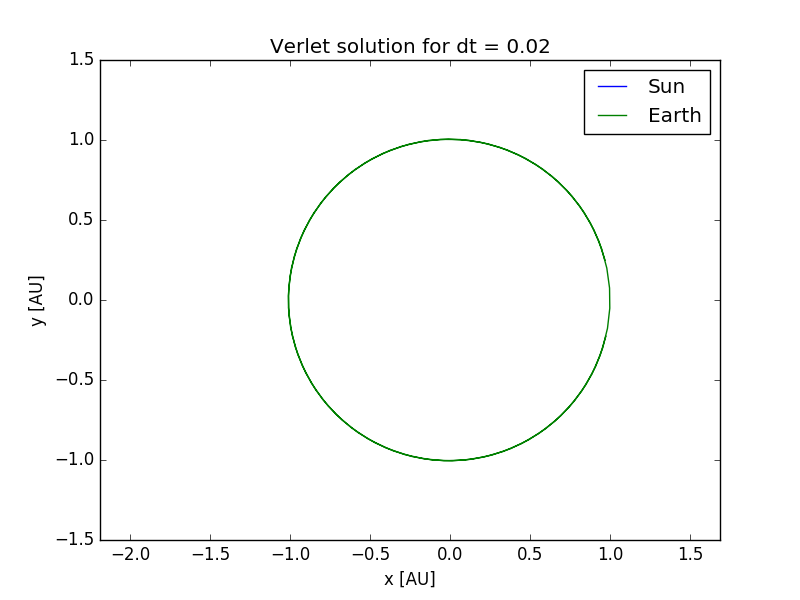
\includegraphics[scale=0.7]{figures/verlet_002}
\caption{The plot shows the simulated orbit of the Earth around the Sun using the velocity-Verlet integration method. The motion is simulated for two years, with $\Delta t = 0.02$ years}
\end{figure}

\begin{figure}[H]
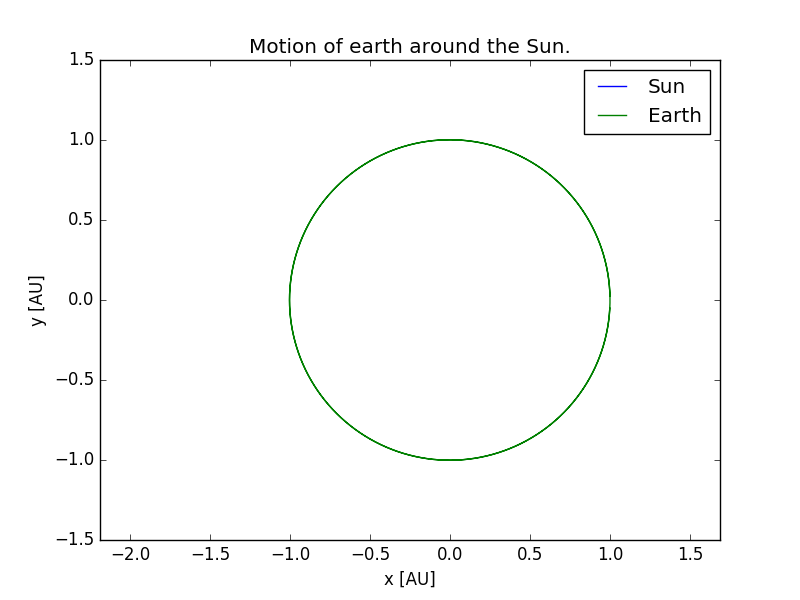
\includegraphics[scale=0.7]{figures/earth_sun_verlet}
\caption{The plot shows the simulated orbit of the Earth around the Sun using the velocity-Verlet integration method. The motion is simulated for two years, with $\Delta t = 0.002$ years.}
\end{figure}

The Euler method does not pass the tests for conservation of kinetic energy, potential energy and angular momentum for $\Delta t = 0.002$\ref{•}

\subsubsection{Escape velocity}\label{results:escape-velocity}
Using the model for the two-body system, a trial and error process of finding the escape velocity
for a planet with initial position 1AU away from the sun was performed. The calculations were
performed using the velocity Verlet method. \ref{fig:escape-no} shows the non-escape case, while
\ref{fig:escape-yes} shows the escaping case.
\begin{figure}[H]\label{fig:escape-no}
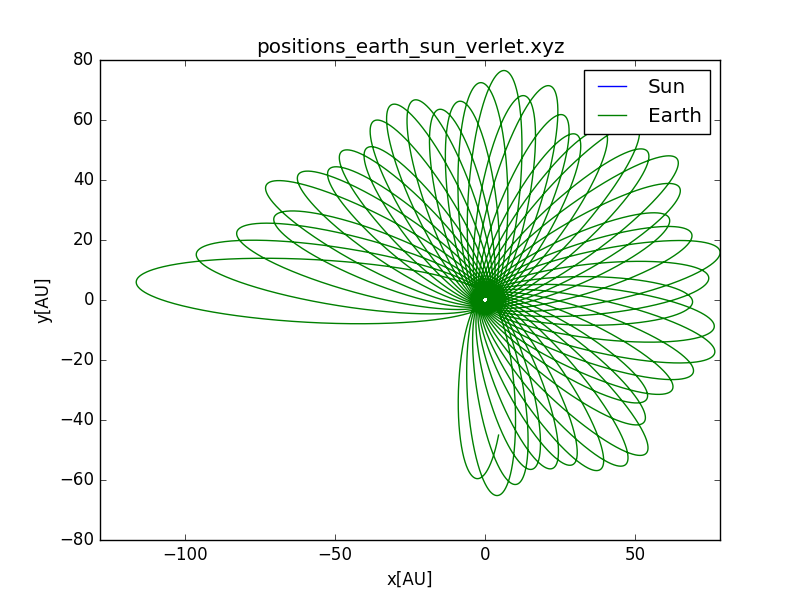
\includegraphics[width=\textwidth]{figures/escape_86}
\caption{The plot shows the position of a planet relative to the sun as a function of time when 
the planet has $v_{init} = 8.6\tfrac{AU}{yr}$}
\end{figure}
\begin{figure}[H]\label{fig:escape-yes}
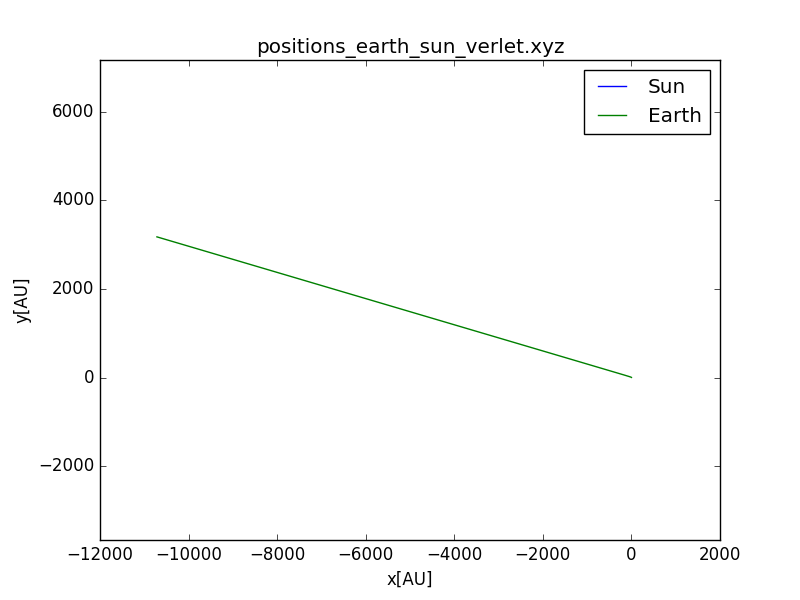
\includegraphics[width=\textwidth]{figures/escape_87}
\caption{The plot shows the position of a planet relative to the sun as a function of time when 
the planet has $v_{init} = 8.7\tfrac{AU}{yr}$}
\end{figure}

\begin{table}
\centering
\caption{Table of execution times for a final time of 10000 years}
\begin{tabular}{|l|l|}
\hline
\textbf{Method}  & \textbf{Time[s]} \\
\hline
Forward Euler   & 0.416121 \\
\hline
Velocity Verlet & 1.17558 \\
\hline
\label{tab:comp-time}
\end{tabular}
\end{table}

\subsection{Three-body system}
Simulating the three body system in which Jupiter acts on earth. The effects of another massive object is explored by adding substantial mass to jupiter to see it's effect on earths trajectory.
 
\begin{figure}[H]
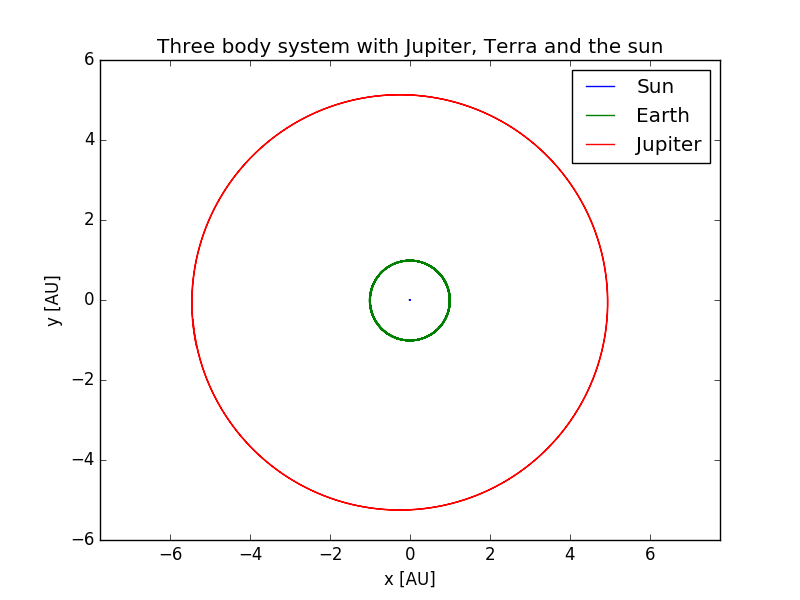
\includegraphics[scale=0.7]{figures/three_body}
\caption{The plot shows the orbit of Earth and Jupiter around the barycentre }\label{fig:three}
\end{figure}

\begin{figure}[H]
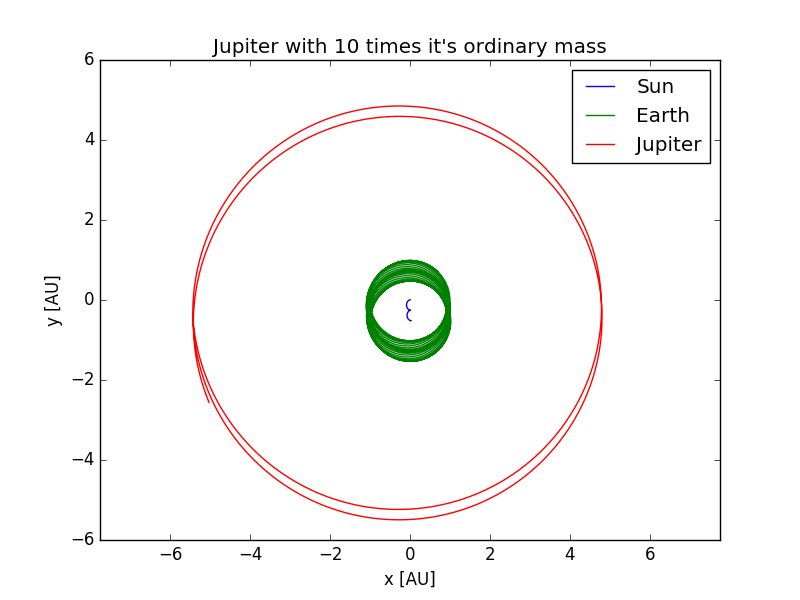
\includegraphics[scale=0.7]{figures/10jup}
\caption{The plot shows the orbit of Earth and Jupiter if Jupiters mass was increased tenfold }\label{fig:ten_j}
\end{figure}

\begin{figure}[H]
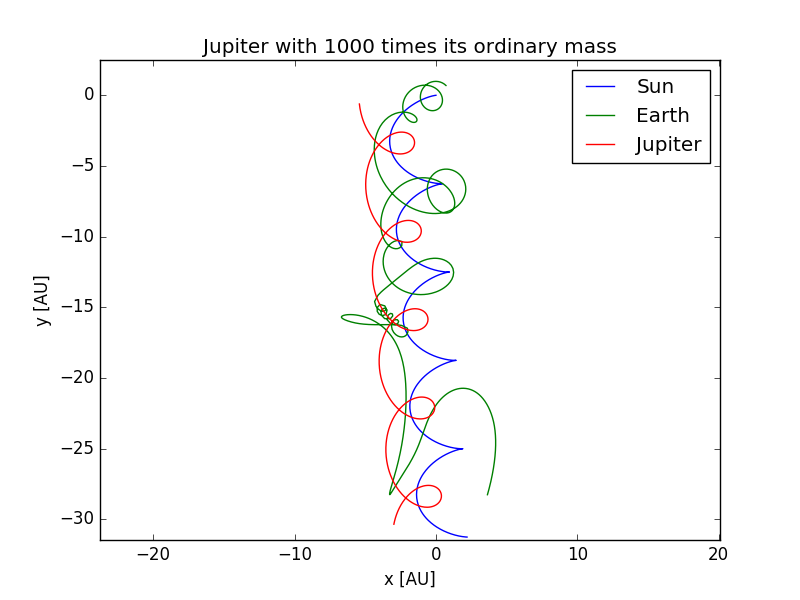
\includegraphics[scale=0.7]{figures/1000jup}
\caption{The plot shows the meandering path of Earth, Jupiter and the Sun if Jupiters mass was increased a thousand fold. Mimicking an unstable orbit of two stars with earth caught in the maelstrom}\label{fig:thous_j}
\end{figure}

\subsection{Full solar system}
\begin{figure}[H]
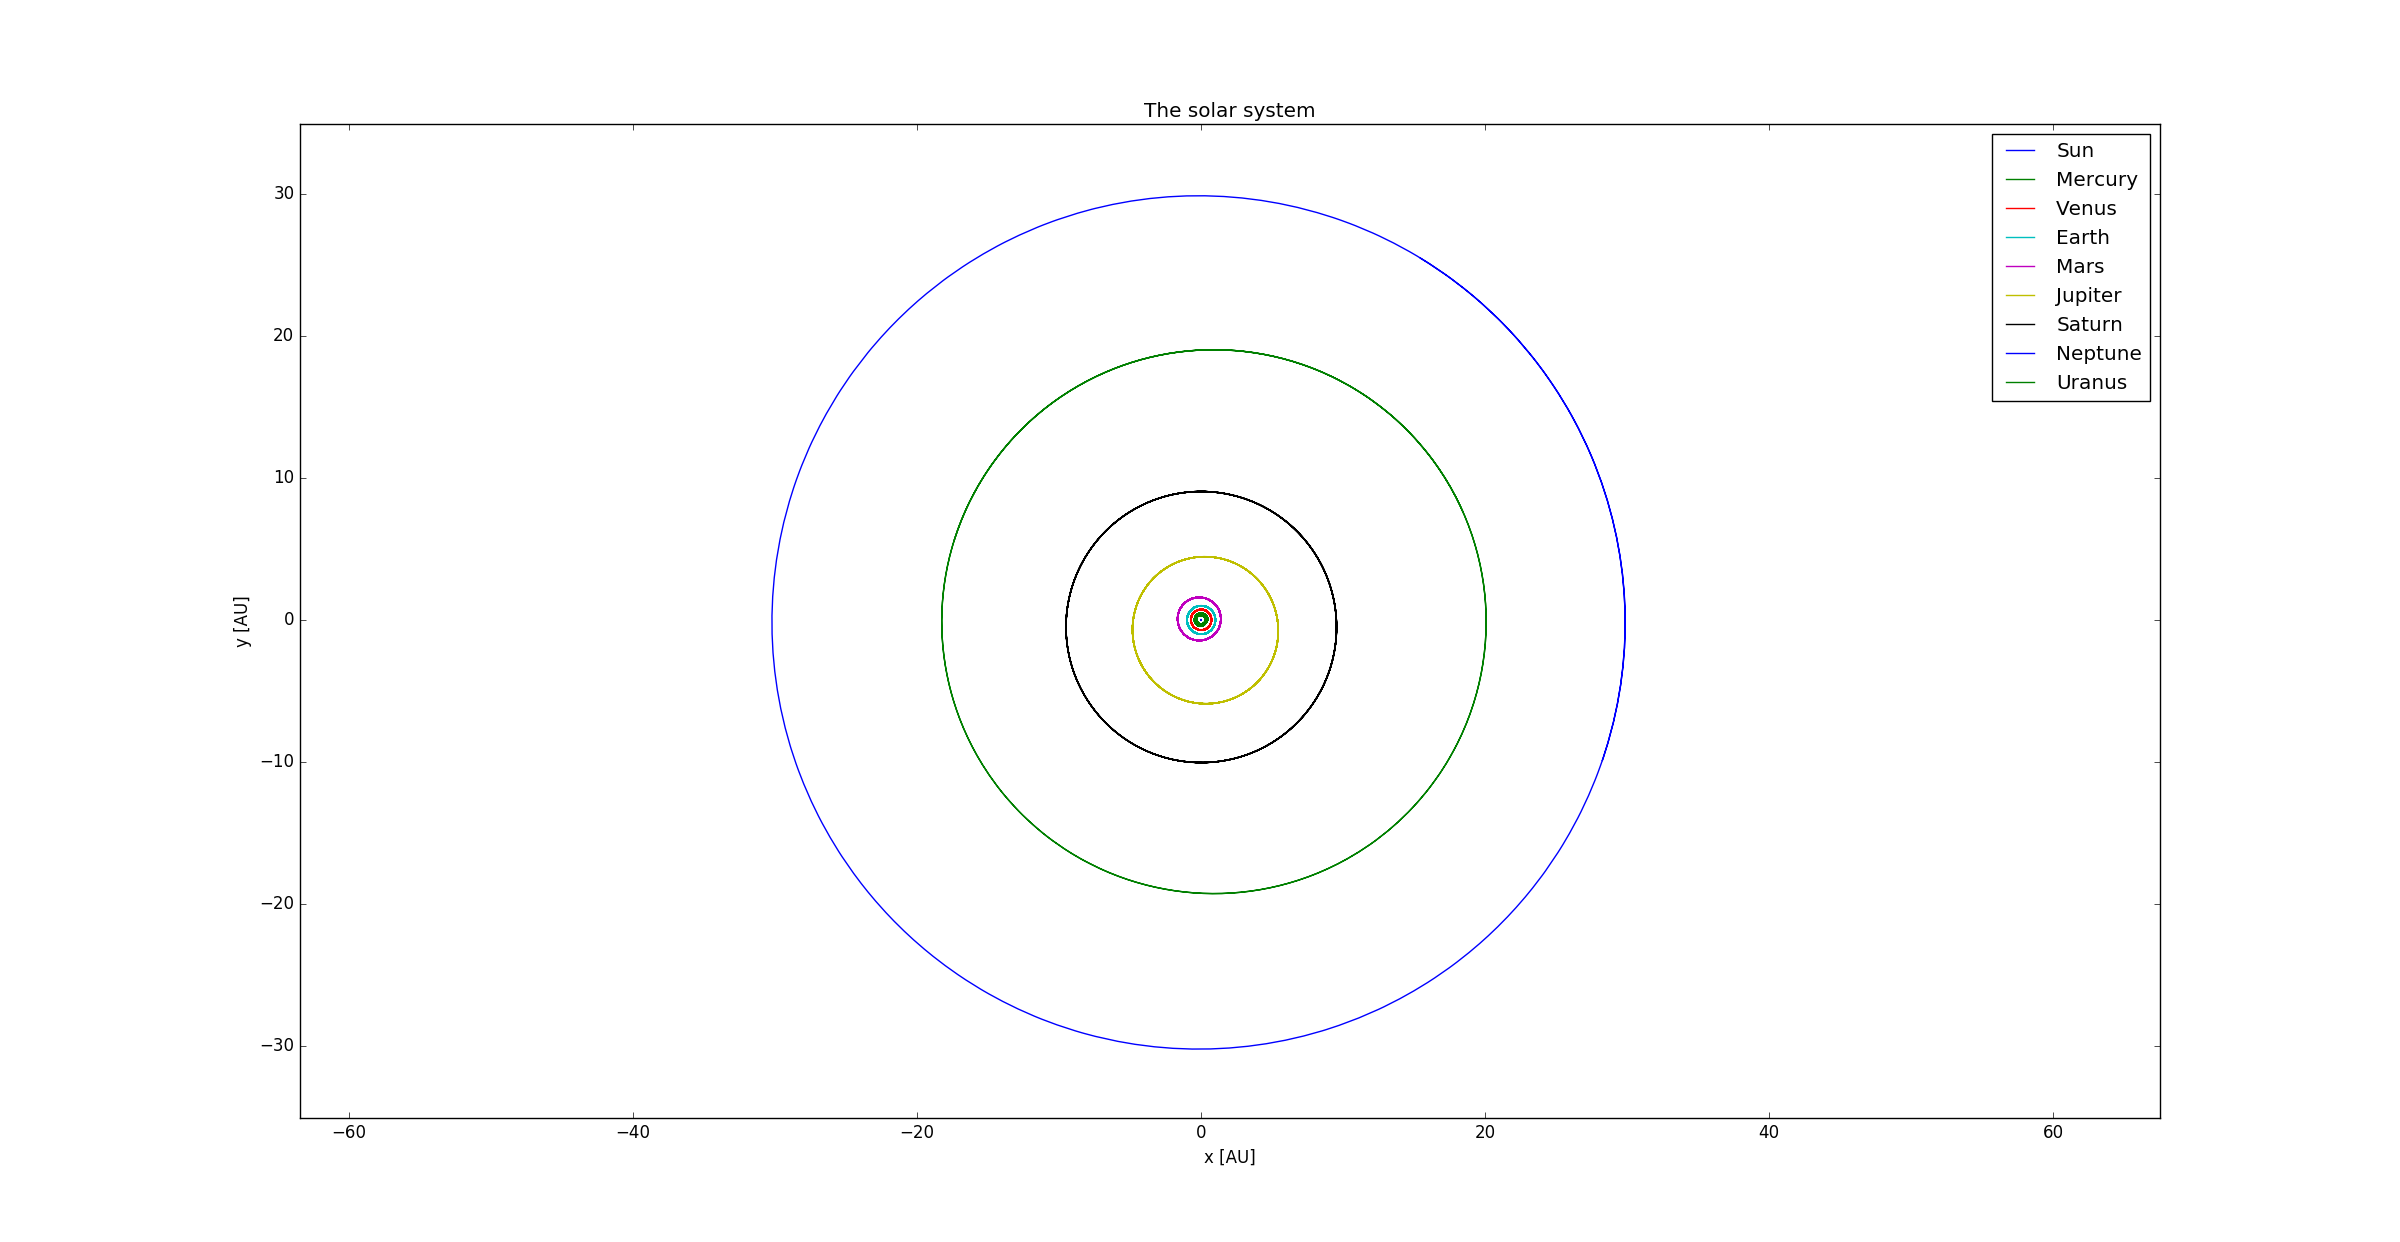
\includegraphics[width=\textwidth]{figures/solarsystem}[h]
\caption{The plot shows the orbit of all the particles in the Solar System around the barycentre}
\end{figure}

